\documentclass{article}

\usepackage{amsmath,amsfonts,amsthm,amssymb}
\usepackage{setspace}
\usepackage{fancyhdr}
\usepackage{lastpage}
\usepackage{chngpage}
\usepackage{hyperref}
\usepackage[usenames,dvipsnames]{color}
\usepackage{graphicx,float,wrapfig}
\usepackage{inconsolata}
\usepackage[round]{natbib}
\usepackage{booktabs}
\usepackage[top=1in,bottom=1in,left=1.5in,right=1.5in]{geometry}
\hypersetup{
  colorlinks = true, % Colours links instead of ugly boxes
  urlcolor = blue, % Colour for external hyperlinks
  linkcolor = blue, % Colour of internal links
  citecolor = blue % Colour of citations
}

%\setlength{\parindent}{0pt}
\setlength{\parskip}{2ex}

% Setup the header and footer
\pagestyle{fancy}
\lhead{Trevor Bekolay, Comprehensive II}
\rhead{\thepage\ of\ \protect\pageref{LastPage}}
\lfoot{}
\cfoot{}
\rfoot{}
\renewcommand\headrulewidth{0.4pt}
\renewcommand\footrulewidth{0pt}

\graphicspath{{figures/}}

% Make title
\title{\bf Biologically inspired methods \\
  in speech recognition and synthesis: \\
  closing the loop}
\date{\today}
\author{{\bf Trevor Bekolay} \\
  Centre for Theoretical Neuroscience, University of Waterloo \\
  Waterloo, ON  N2L 3G1}

\begin{document}

\maketitle

\begin{abstract}
  I propose to build a system that recognizes
  a small vocabulary of words,
  and synthesizes that same vocabulary
  with no prior knowledge.
  The system will use biologically inspired methods:
  the speech recognizer will use a
  human auditory periphery model
  to transduce audio signals,
  and the synthesizer will
  produce audio signals
  using a model of the human vocal tract
  with 23 articulators.
  The two systems will have
  reciprocal connections,
  closing the perception-action loop
  and providing a starting point for
  larger systems combining
  sophisticated hierarchical
  recognition and synthesis systems.
\end{abstract}

\section{Introduction}
\label{sec:intro}

The human auditory system is an
amazing product of evolution;
we are able to utter hundreds of phonemes,
which we blend together---without pauses---into
sentences that we recognize effortlessly,
despite huge variations in the
volume and intelligibility of
those phonemes,
and even in noisy rooms with
dozens of overlapping speakers.
Attempts to replicate the human auditory system
in computers have resulted in
speech recognition systems with
high accuracy in certain environments,
and speech synthesizers that
can voice novel utterances
in a recognizable and
(mostly) natural way.
Unlike the human auditory system, however,
speech recognition systems
and speech synthesis systems
are separate non-interacting systems;
there is currently no system
that listens to the audio it produces
and adapts itself to recognize
and synthesize better speech over time.

My project aims to close this loop
and show that computational
recognition and synthesis systems
can be used to improve each other over time,
as biological systems do.
I will also exploit how biological systems
represent and transform information
to pass data between the interacting systems
in a form that can be understood by both.
Specifically, I will build the interacting
recognition and synthesis systems
as spiking neural networks using the
methods of the Neural Engineering Framework.
In doing so, I hope to make contributions
to speech science by showing that
recognition and synthesis systems
can improve each other,
and to neuroscience by providing
a concrete hypothesis of how
the human auditory system
might be organized
that can be used to generate
experimentally testable predictions.

\section{Background}
\label{sec:background}

\subsection{Speech recognition}
\label{subsec:recognition}

Automatic speech recognition
is a large and still growing field
that has acted as a test bed
for new AI techniques for decades,
due to the allure of enabling
interactions with computers
using the same means
as humans interact with other humans.
Speech recognition can be formalized
with the following equation.
\begin{equation}
  \max_W P(W|O) = \max_W P(O|W) P(W),
\end{equation}
where $W$ is a sequence of words,
and $O$ is an audio waveform.
In this formalism, the speech recognition problem
is to find the most likely sequence of words
given some audio waveform.
Applying Bayes' rule, we can find
this sequence of words
if we know the probability
of some sequence of words occurring
in the target language,
and the distribution of audio waveforms
given some sequence of words.
In the literature, these two terms
are sometimes given explicit names.
The probabilities of a word sequence
occurring in a target language,
$P(W)$, is called the \textit{language model}
and the distribution of waveforms
given a word sequence, $P(O|W)$,
is called the \textit{acoustic model}.

In practice, these probability distributions
are far too large to compute;
instead, the problem of speech recognition
is broken down into several subproblems
that are solved in sequence,
resulting in a speech recognition ``pipeline.''
While some techniques may span several levels
of the pipeline, at its finest granularity,
there are six levels to the pipeline,
as shown in Figure~\ref{fig:recognition}.

\begin{figure}
  \begin{center}
    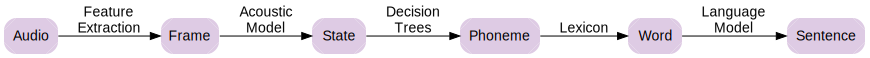
\includegraphics[width=1.0\linewidth]{recognition}
  \end{center}
  \caption{Pipeline used in many speech recognition systems.}
  \label{fig:recognition}
\end{figure}

The pipeline begins with the \textit{audio waveform}.
This one-dimensional signal is transformed
into a sequence of \textit{audio frames}
in a process typically called feature extraction.
Speech researchers have followed
biology by using the frequency spectrum
of the time-varying audio waveform
as the primary feature to be extracted.
The frequency components of the waveform
over a small time-window are often compressed,
resulting in each audio frame consisting of
a tractable number of coefficients
that describe the frequency components
of a slice of the audio waveform
(typically around 10 milliseconds of audio).
This transformation is typically done
with Fourier analysis,
which is sometimes sampled
on the Mel scale
(which is proportional to
log frequency and is inspired
by human perceptual studies; \citealp{stevens1937,furui1981}).
However, more sophisticated methods
such as Perceptual Linear Prediction \citep{hermansky1990},
and Linear Predictive Coding \citep{oshaughnessy1988},
have been used to construct audio frames from a waveform.

One or more audio frames are then mapped
to a \textit{state}
in a Hidden Markov Model (HMM).
This transformation is also called
\textit{acoustic modeling},
as we are building a statistical model
of the subphonemic HMM states
given the audio frame.
The first generation of successful
speech recognition systems
used Gaussian Mixture Models
to do efficient acoustic modeling
(e.g., \citealp{reynolds1995}).
However, modern speech recognition systems,
such as those used by Google,
use neural networks
(specifically, neural networks trained with deep learning)
for acoustic modeling
(e.g., \citealp{jaitly2012}).

Sequences of HMM states are transformed
into \textit{phonemes}.
There can be many HMM states
for a single phoneme \citep{rabiner1989}.
Phonemes are the smallest atoms of speech
studied in linguistics,
as they can be discriminated consciously by humans.
Mapping from states to phonemes
is typically done through a composition operation
by a finite state transducer (FST; \citealp{mohri2002}).
FSTs are heavily used in the higher levels
of speech recognition,
as they offer a mathematical formalism
that can be manipulated with efficient algorithms
\citep{mohri2000}.

Phonemes are composed to form \textit{words}.
The phonemes that make up each word
can be looked up
in the target language's \textit{lexicon}.
In practice, the lexicon is often encoded
in a finite state transducer
\citep{mohri2002}.

Words are composed to form \textit{sentences}.
While this starts to encroach
on higher-level features of language,
such as syntax,
most speech recognition systems
use simple statistical techniques
to determine if a sequence of words
forms a sentence.
However, approaches that combine
speech recognition and natural language processing
are the subject of significant
academic and industrial research
(e.g., \citealp{sagae2009}).

Little is known about the neurobiology
of speech recognition;
while several auditory pathways have been identified
in the human brain \citep{scott2003},
it is unclear if those pathways map onto
the speech recognition pipeline
used in artificial intelligence.
However, the first stage of the pipeline,
the mapping from audio waveforms
to audio frames, was originally inspired
by the auditory periphery system
in the brain.
Recent developments in auditory periphery modeling
have yet to be compared to the methods used
in artificial speech recognition,
and it may be possible that
these auditory periphery models
provide a better starting point
for the remaining steps in the pipeline
than existing techniques.

\subsection{Auditory periphery modelling}
\label{subsec:periphery}

While the functions of brain areas
associated with auditory processing
are largely unknown,
the auditory periphery is well understood.
Briefly, the auditory periphery
is responsible for sensing pressure waves
in the air and transducing them into
neural signals that we perceive as sound.
As seen in Figure~\ref{fig:anatomy}\footnote{Figure~\ref{fig:anatomy}
  adapted from
  \url{http://commons.wikimedia.org/wiki/File:Anatomy_of_the_Human_Ear.svg}
  and \url{http://en.academic.ru/dic.nsf/enwiki/1472779}},
air pressure waves are funneled into the auditory canal,
causing the tympanic membrane (eardrum)
to vibrate, which causes the stapes
to move in and out of the oval window of the cochlea.
Inside the cochlea, the movement of the stapes
disturbs fluid around the basilar membrane,
causing it to deform at specific points
depending on the frequency of the movement
of the stapes; higher frequency movements
cause deformation at the base of the basilar membrane,
and low frequency movements cause deformation
at the apex of the basilar membrane.
Hair cells lie on top of the basilar membrane
and touch the tectorial membrane.
As the basilar membrane is deformed,
the hair cells lie against
the tectorial membrane at different angles,
which cause different amounts of ions
to flow into the hair cell.
This directly controls the membrane potential
of the hair cells,
which is communicated
to the brain through cochlear nerve fibers.
Note that the hair cells exhibit graded potentials;
that is, they do not fire action potentials.
The hair cells synapse with spiral ganglion neurons,
whose axons form the auditory nerve
(also known as the cochlear nerve).
Unlike hair cells, spiral ganglion cells
communicate via action potentials.

\begin{figure}
  \begin{center}
    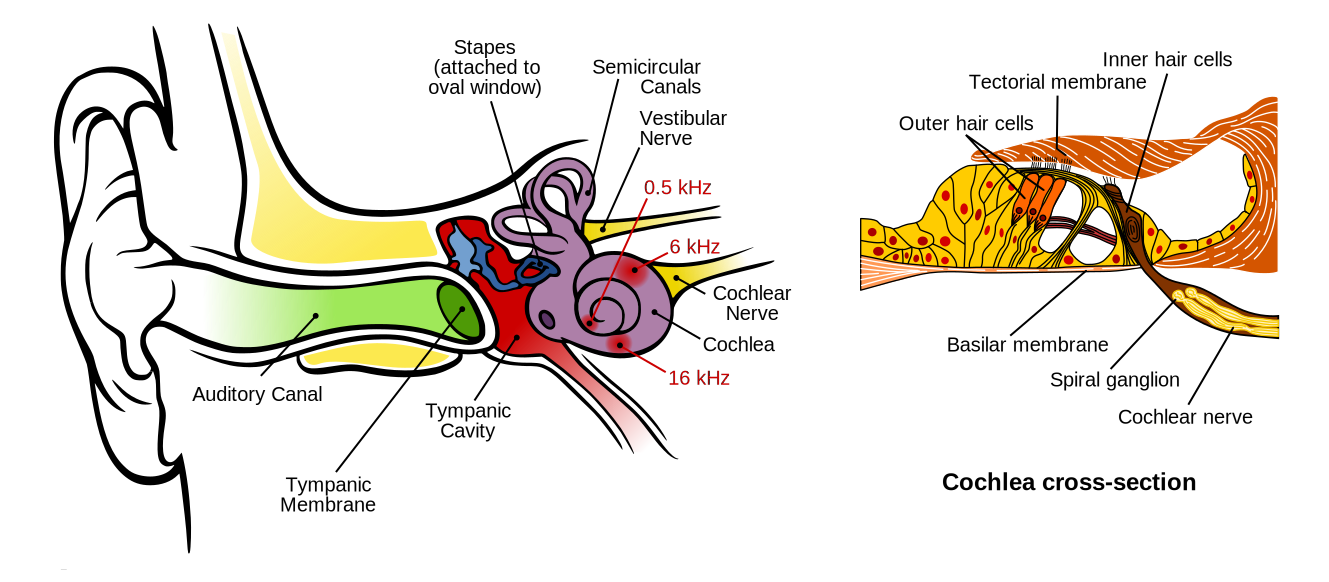
\includegraphics[width=1\linewidth]{periphery-anatomy}
  \end{center}
  \caption{Anatomy of the human auditory periphery.
    (Left) A view of the outer and inner ear.
    Pressure waves travel down the auditory canal,
    causing the tympanic membrane to vibrate.
    Those vibrations translate to movements of the stapes,
    causing disturbances in the fluid of the cochlea.
    Those disturbances cause parts of the cochlea
    to be deformed; high-frequency sounds cause
    deformations at the base of the cochlea,
    while low-frequency sounds cause deformations
    at the apex (middle) of the cochlea.
    (Right) Cross-section of the cochlea.
    Hair cells lie on top of the basilar membrane,
    which is deformed by the movement of the stapes.
    As outer and inner hair cells push against the
    tectorial membrane at different angles,
    ion channels flow into the hair cell,
    which is communicated to spiral ganglion cells.
    Spiral ganglion cells send action potentials
    through the cochlear nerve to the brain.}
  \label{fig:anatomy}
\end{figure}

While the basic function of the auditory periphery
is to separate the incoming vibrations
into its frequency components,
as speech recognition systems do,
the actual transformation is significantly
more complicated than that.
Frequency components are nonlinearly weighted.
The incoming signal is amplified
if its amplitude is low,
but at a certain volume transitions
to a non-amplified state,
resulting in complicated dynamics
at the transition point.
These and several other nonlinearities
make auditory periphery modeling
significantly more complicated
than just Fourier analysis.

\subsubsection{Zilany model}
\label{subsec:zilany}

A computational model proposed originally by
Bruce, Sachs \& Young
and later extended by Zilany, Bruce, Nelson, \& Carney
has been able to replicate
many of the peculiarities
of the biological auditory periphery
\citep{bruce2003,zilany2006,zilany2007,zilany2009,zilany2014},
and has been used in cochlear implants
due to its ability to produce
similar signals as biological hair cells.
We will refer to this as the
Zilany model in the remainder of this proposal.

The Zilany model,
summarized in Figure~\ref{fig:zilany},
consists of a series
of interacting nonlinear filters
which produce a membrane potential
similar to that produced
by inner hair cells along the basilar membrane.
This is fed into a synapse model and spike generator
that emulates spiral ganglion cells
and produces the action potentials
that travel along the auditory nerve.

\begin{figure}
  \begin{center}
    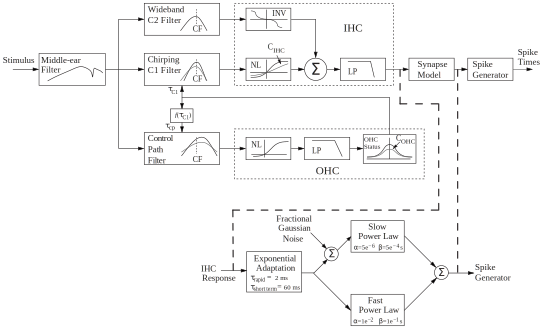
\includegraphics[width=1\linewidth]{zilany}
  \end{center}
  \caption{Zilany model of the human auditory periphery
    \citep{zilany2006}. See text for details.}
  \label{fig:zilany}
\end{figure}

The instantaneous pressure waveform
(i.e., the audio input)
goes through a middle-ear filter,
whose output goes through three sets of filters
that are evaluated in parallel:
the C1, C2 and control path filters.
The middle-ear filter is a fifth order digital filter.
The control path is responsible for
setting the $\tau_{C1}$ time constant,
which affects the gain and bandwidth
of the C1 filter.
$\tau_{C1}$ is determined by
a series of nonlinear
(gammatone, Boltzmann)
and low-pass filters.
The C1 and C2 filters are
complex functions with three poles
(i.e., frequencies for which the
value of the function goes to infinity)
and one zero (i.e., a frequency
for which the value of the function goes to zero).
The locations of the poles and zero
are determined by
several parameters, including
the tuning properties of
the hair cell being simulated,
and its characteristic frequency,
which partially determines the cell's
tuning properties.
The C1 filter is responsible for most
low to medium frequency responses,
modeling both inner and outer hair cell
activity, resulting in a chirp filter.
The C2 filter is responsible
for high frequency responses,
modeling inner hair cell activity
with a wideband filter;
the C2 filter is identical
to the broadest possible C1 filter,
which occurs when the outer hair cells
are completely impaired.
Finally, the C1 and C2 filters
are transduced to a voltage response,
summed together, and low-pass filtered
to obtain the final output voltage
of the inner hair cells.

The resulting voltage from the inner hair cell
is then communicated to
a spiral ganglion-like spike generator
through the IHC-AN synapse.
This synapse exhibits adaptation dynamics
on at least three time scales:
rapid adaptation on the scale of milliseconds,
short-term adaptation on the scale of tens of milliseconds,
and slow adaptation on the scale of seconds.
Zilany et al. model each time scale explicitly.
On the shortest time scale,
adaptation is exponential.
Exponential adaptation occurs naturally
through simulating the diffusion
of three stores of neurotransmitter
across the synaptic cleft.
On the medium and long timescales,
power-law adaptation is directly computed
by convolving a power-law kernel with
the history of prior responses;
the parameters of the kernel
are larger on the medium timescale
compared to the long timescale.
The results of the three timescales
are combined to give the output
in terms of the spontaneous rate
(spikes per second) of the cell being simulated.

The spontaneous rate,
as determined by the synapse model,
is mapped to spike times
through a nonhomogeneous Poisson process
modified to include refractory effects
\citep{zhang2001}.

\subsection{Speech synthesis}
\label{subsec:synthesis}

Speech synthesis is the converse
of speech recognition;
given a sequence of words,
produce an audio waveform
that resembles a human
voicing that sequence of words.
The pipeline for synthesis is very similar
to the pipeline for recognition,
only in reverse:
sentences are broken down into words,
which are broken down into
their underlying phonemes.
This is typically called the
``frontend'' of a speech synthesis system.
The phonemes are then either
directly converted into audio waveforms,
or further broken down into
smaller states which are converted to audio waveforms.
This is typically called the ``backend''
of a speech synthesis system.

While speech recognition
has seen significant advances
and commercial success recently,
speech synthesis remains
unsatisfactory to the general public
despite recent advances.
Modern speech synthesizers can
produce natural-sounding speech,
but that speech is inflexible
and cannot be modified
to reflect the speaker's
emotional state or speaking style.
Synthesis techniques
that are more flexible exist,
but are computationally intensive,
and sound ``robotic,''
or too perfect,
due to the way in which
speech is produced.

Currently, the dominant speech synthesis
methods is concatenative (or unit selection) synthesis
\citep{hunt1996}.
In concatenative synthesis, waveforms are generated
by selecting and concatenating audio samples
from a large database of recorded sounds
(called ``units,'' which are typically phonemes,
but may be shorter to capture coarticulation).
Since the units are recordings of real speech,
the result sounds natural.
Audio databases typically contain samples with
varying prosodic characteristics
(rhythm, stress, intonation)
allowing for words to be synthesized
using the underlying units
with the desired prosodic characteristics
(as long as units with those characteristics
have been recorded).
Machine learning techniques
are employed to efficiently search
the database of units and combine
the units together
(e.g., HMMs and Viterbi search,
as are used in speech recognition).
While the results are generally good
(concatenative synthesis is used in
the majority of commercially available
text-to-speech systems\footnote{See
  \url{http://www.theverge.com/2013/9/17/4596374/machine-language-how-siri-found-its-voice}.})
this technique is limited to the corpus
of sounds available in the database,
which can be costly to record.
Additionally, there can be discontinuities
in the transition from one unit
to the next, making the recorded
voice sample sound artificial.
Attempts to modify the concatenated
samples after the fact,
to change its prosodic characteristics,
for example, often require
spectral transformations that also
result in unnatural-sounding speech
\citep{schroder2001}.

Advances in computing power
have made statistical parametric synthesis
techniques viable \citep{zen2009}.
While concatenative synthesis
cobbles together speech using existing speech,
statistical parametric synthesis
addresses speech synthesis
as a generative statistical problem,
much in the way that
the speech recognition formalism does.
Like concatenative synthesis,
a large database of recorded speech is necessary,
but instead of using
raw samples from that database,
the database is used to generate
a set of model parameters.
The problem of speech synthesis
is represented as
\begin{equation}
  \hat{o} = \arg \max_o P(o|W, \hat{\lambda}),
\end{equation}
where $o$ is a set of speech parameters,
$W$ is a sequence of words,
and $\hat{\lambda}$ is a set of model parameters
resulting from training on the speech database.
The appropriate speech parameters
for the given word sequence, $\hat{o}$,
is fed through a series of filters
to generate synthesized speech.

The most common method of implementing
statistical parametric synthesis
is to use an elaborate set of HMMs,
working at many different levels
and in parallel to model
all of the features necessary to produce
intelligible speech.
These features sets are significantly
more complicated than those
used in speech recognition;
in recognition, phonetic, prosodic,
and other contextual cues
can be collapsed into single HMM states,
whereas in synthesis,
all of these states must be explicitly tracked.
In one system \citep{zen2007},
there over a hundred parameters to be modeled.
Like similar techniques in speech recognition,
deep neural networks have begun
to replace HMMs, with promising results
\citep{zen2013}.
Despite these advances, concatenative systems
were still judged the most natural
at the 2012 Blizzard Challenge
(\citealp{kinga2012};
2013 results not available at this time).

\subsection{Articulatory speech synthesis}
\label{subsec:articulatory}

The most flexible approach to speech synthesis
is articulatory speech synthesis.
Articulatory synthesis systems generate
audio waveforms by simulating
airflow through the human vocal tract.
While this method is
the most closely tied to biology,
and was used in the first fully automatic
text-to-speech synthesizer \citep{klatt1987},
its computational complexity
and artificial sounding results
have hindered its adoption
among academics and industry.
Additionally, accurate simulation
requires intricate knowledge
of how the human vocal tract
produces sounds,
which at present is incomplete.
However, unlike other methods,
articulatory speech synthesis
is able to test theories
resulting from the biological exploration
of sound production
and produce novel predictions.

Generally, articulatory speech synthesizers
consist of three models
\citep{kroger2009}.
The first is a \textit{control model},
which generates vocal tract movements
by determining the desired positions
of the articulators in the vocal tract
(i.e., the degrees of freedom in the control problem).
The second is a \textit{vocal tract model},
which converts movements, or desired positions,
into vocal tract geometries in continuous time.
The third is an \textit{acoustic model},
which converts the geometries of the vocal tract
into acoustic signals (i.e., audio waveforms).
Each module has several classes of implementations.

One class of control models used in
articulatory speech synthesis
are segmental control models,
which work on a set of goals and constraints
\citep{kroger1992}.
Given a phonological description
of the utterance to be synthesized,
segmental control models
produce a set of timestamps
(when a phoneme is to be voiced)
and a set of goals for some,
but not necessarily all,
of the articulators.
For example, to voice an \textit{a},
a segmental control model might say
that the \textit{a} starts at 0 ms
and ends at 100 ms,
and that the glottal aperture
must be at position 10
for that entire time window,
but that the tongue tip
should aim to reach position 0
at some point in that time window.
By specifying hard and soft constraints
on the vocal tract model,
segmental control can produce
realistic transitions between
phonemes simply by allowing
non-essential articulators to
remain in their current positions.

Another class of control models are
action based control models,
also known as gestural control models,
which define a set of discrete motor actions
(i.e., motor primitives in motor control literature)
that are combined to produce sounds according
to a phonemic and prosodic description
\citep{birkholz2006}.
This leads to several levels of description.
At the highest level,
the description to voice an \textit{a}
might be
``close the glottis
and open the velopharyngeal valve.''
This gets mapped down to a
high level motor plan,
which defines when the ``glottal closing''
and ``velopharyngeal valve opening''
actions occur and for how long.
This then is mapped down
to a lower level phonetic articulatory description
(using inverse dynamics)
that defines how each articulator
moves over time.

The control model is tightly coupled
with the vocal tract model,
since the vocal tract model defines
the articulators that can be controlled.
It also typically provides some clue
for what articulator values
are appropriate for the
phoneme being synthesized.

One class of vocal tract models
are statistical models,
which extract relevant characteristics
from a large set of data,
mostly magnetic resonance imaging (MRI)
paired with audio recordings
(e.g., \citealp{badin2002}).
A full three-dimensional representation
of the patient's vocal tract
can be reconstructed with sufficient data,
and by using dimensionality reduction techniques,
the articulatory control parameters
can be of relatively low dimensionality
while still producing a full
3D representation of a vocal tract.

\begin{wrapfigure}{l}{0.421\textwidth}
  \vspace{-30pt}
  \begin{center}
    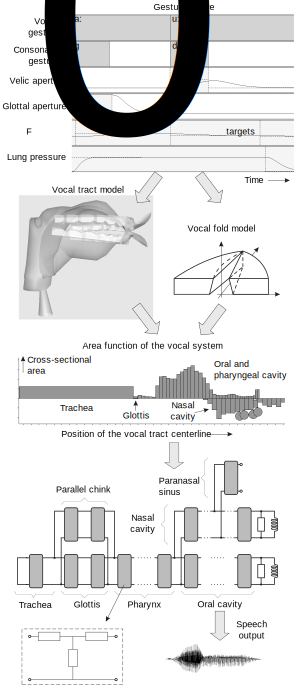
\includegraphics[width=0.42\textwidth]{birkholz}
  \end{center}
  \vspace{-12pt}
  \caption{Birkholz articulatory synthesizer
    \citep{birkholz2013}. See text for details.}
  \label{fig:birkholz}
  \vspace{-20pt}
\end{wrapfigure}

Another class of vocal tract models
are biomechanical models,
which attempt to fully reconstruct
the physiology of the vocal tract
(e.g., \citealp{dang2004}).
This type of model is similar
to the statistical model,
in that MRI and other anatomical measurements
are used to develop a 3D representation
of the vocal tract.
However, instead of statistically
reducing the dimensionality
to determine the degrees of freedom
available to the control system,
these models also model how
muscle activations affect the shape
of the vocal tract
and use each muscle
as a degree of freedom.

A final class of vocal tract models
are geometric models,
which generalize the overall
shapes observed in
MRI and anatomical studies
(e.g., \citep{mermelstein1973}).
A set of parameters
are used to generate a 3D model
of a vocal tract,
which has a set of articulators.
While these models are typically
less detailed than those
generated from precise
measurements of one subject's vocal tract,
it can be used to generate vocal tracts
from different subjects
(both male and female).
The parameters of the model
can therefore be tuned to a specific speaker,
though the resulting vocal tract
will not be as detailed
as one determined solely through
measurements of that speaker.

Finally, the acoustic model takes
a vocal tract representation
and simulates the airflow from
the lungs, through the vocal tract,
to the air pressure coming out of the mouth.
These models typically relate
the vocal tract to some other
device with known physics.
One set of models treat the vocal tract
as an analog transmission line,
similar to models simulating
arterial blood flow \citep{meyer1989}.
Another set of models treat the vocal tract
as an analog electrical circuit
\citep{maeda1982}.
A final set of models,
called finite element wave propagation models,
explicitly model the air pressure wave
as it travels through each section
of the vocal tract \citep{elmasri1996}.
Hybrid technique combine one
of the above techniques
with an analogous transformation
in the frequency domain for added accuracy
\citep{sondhi1987}.
Within these systems, the glottis model
and the noise generated
by air turbulence can be changed
to modify the final synthesized audio waveform.

\clearpage

\begin{wrapfigure}{l}{0.41\textwidth}
  \vspace{-30pt}
  \begin{center}
    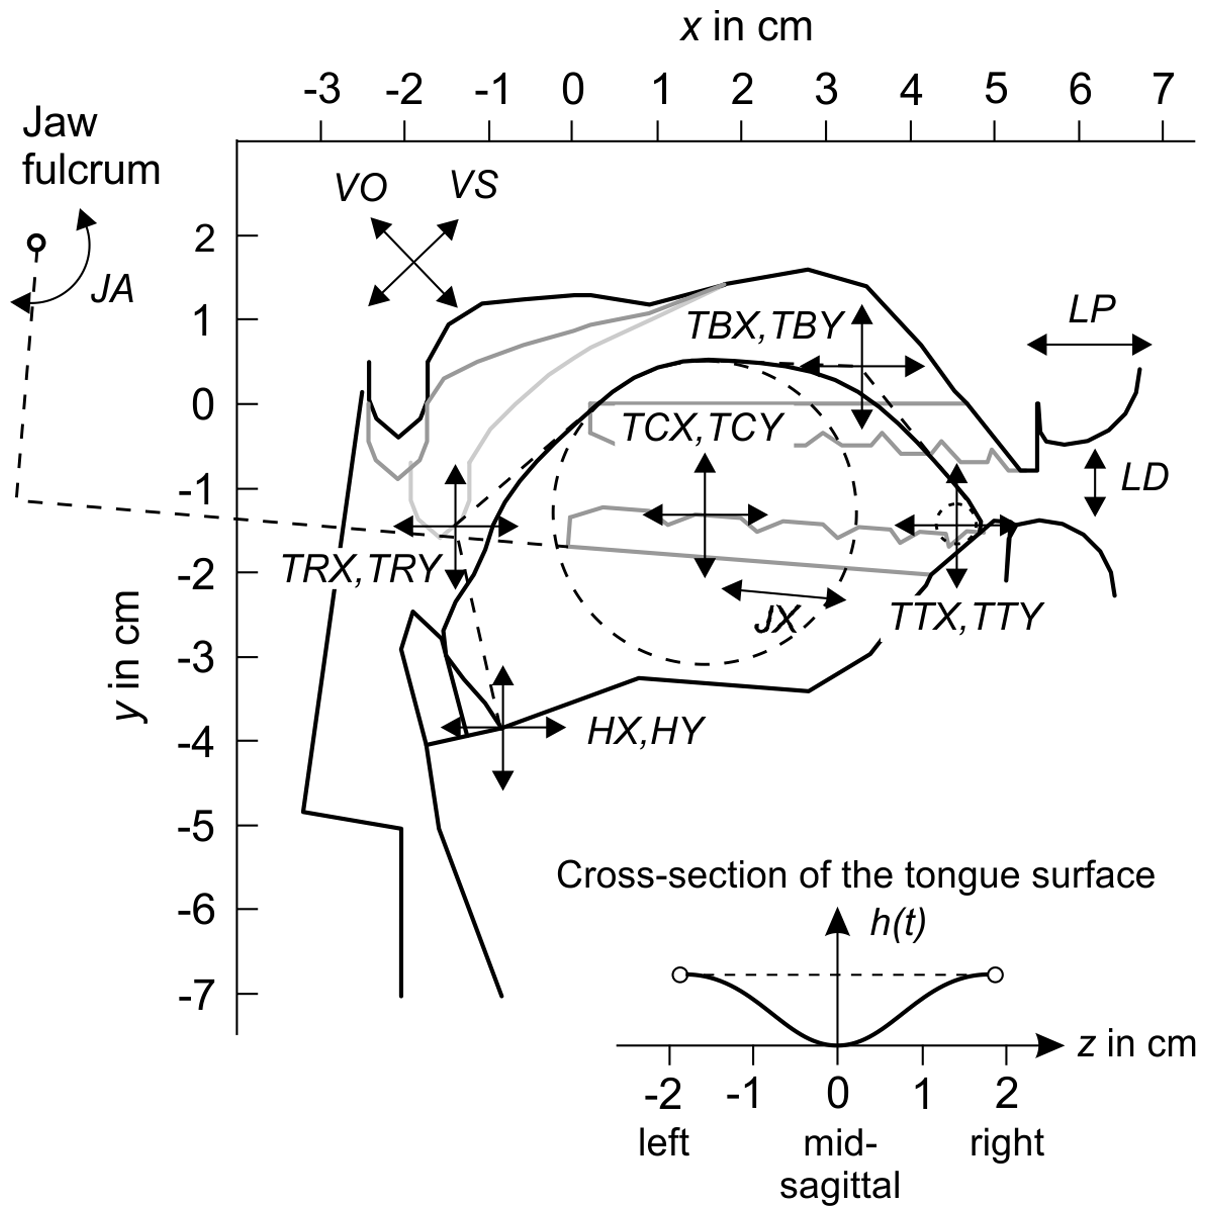
\includegraphics[width=0.41\textwidth]{birholz-params}
  \end{center}
  \vspace{-24pt}
\end{wrapfigure}

\subsubsection{Birkholz synthesizer}
\label{subsec:birkholz}

One of the most successful articulatory
synthesizers\footnote{An early version of the synthesizer
  came second in a singing challenge
  at Interspeech 2007; results available at
  \url{http://www.interspeech2007.org/Technical/synthesis_of_singing_challenge.php}.}
is one by Birtkholz et al,
(available at \url{http://www.vocaltractlab.de/};
\citealp{birkholz2013}).
We will refer to it as the Birkholz synthesizer.
The Birkholz synthesizer uses
an analog electrical circuit transmission line
for generating acoustics,
a geometric model for the vocal tract,
and an action based control model.

While the full details of the acoustic model
and the vocal tract model are not
essential for the work proposed here,
it is useful to note
the 23 degrees of freedom
being controlled by Birkholz's
action based control model.

\begin{tabular}{llrrl}
\toprule
{\bf Name} & {\bf Description} & {\bf Min.} & {\bf Max} & {\bf Unit} \\
\midrule
$HX$ & Horizontal hyoid position & 0.0 & 1.0 & \\
$HY$ & Vertical hyoid position & -6.0 & -3.4 & cm \\
$JX$ & Horizontal jaw displacement & -0.5 & 0.0 & cm \\
$JA$ & Jaw angle & -7.0 & 0.0 & deg \\
$LP$ & Lip protrusion & -1.0 & 1.0 & \\
$LD$ & Vertical lip distance & -2.0 & 4.0 & cm \\
$VS$ & Velum shape & 0.0 & 1.0 & \\
$VO$ & Velic opening & -0.1 & 1.0 & \\
$TCX$ & Tongue body center X & -3.0 & 4.0 & cm \\
$TCY$ & Tongue body center Y & -3.0 & 1.0 & cm \\
$TTX$ & Tongue tip X & 1.5 & 5.5 & cm \\
$TTY$ & Tongue tip Y & -3.0 & 2.5 & cm \\
$TBX$ & Tongue blade X & -3.0 & 4.0 & cm \\
$TBY$ & Tongue blade Y & -3.0 & 5.0 & cm \\
$TRX$ & Tongue root X & -4.0 & 2.0 & cm \\
$TRY$ & Tongue root Y & -6.0 & 0.0 & cm \\
$TS1$ & Tongue side elevation 1 & -1.4 & 1.4 & cm \\
$TS2$ & Tongue side elevation 2 & -1.4 & 1.4 & cm \\
$TS3$ & Tongue side elevation 3 & -1.4 & 1.4 & cm \\
$TS4$ & Tongue side elevation 4 & -1.4 & 1.4 & cm \\
$MA1$ & Minimum area tongue back region & 0.0 & 0.3 & cm$^2$ \\
$MA2$ & Minimum area tongue tip region & 0.0 & 0.3 & cm$^2$ \\
$MA3$ & Minimum area lip region & 0.0 & 0.3 & cm$^2$ \\
\bottomrule
\end{tabular}

In \citet{birkholz2013}, the actions generated from
the phonetic and prosodic representation
are mapped to changes in
the 23-dimensional control parameters
through analysis of MRI and dynamic MRI recordings
of a single speaker.
From that starting point,
each vowel phoneme was optimized
by minimizing the difference
between the simulated formants
and the speaker's formants\footnote{A
speech formant is a frequency that
has a high amplitude for a specific sound.
Three such formants have been identified
for most phonemes, though usually only the first
two are necessary to uniquely identify
a phoneme; for example, the long \textit{e}
vowel sound (as in fr\textit{ee})
can be uniquely identified with
formants $f_1=240$ Hz and $f_2=2400$ Hz.}
The optimization
was done using a greedy hill-climbing algorithm
in which each degree of freedom in
the control signal for a given vowel
was varied positively and negatively
and the formant difference was evaluated
until a local minimum was found.

Despite this optimization procedure
being relatively simple,
subjective error rates dropped dramatically,
pointing to the possibility
of greatly improved synthesis
by using more sophisticated optimization techniques.

\subsection{Motor control}
\label{subsec:motor-control}

Articulatory speech synthesis
can be thought of as a
general motor control problem;
in the case of the Birkholz synthesizer,
the plant is the vocal tract model,
which has 23 degrees of freedom.
However, as an additional difficulty
above and beyond general motor control,
the position of the plant is
not necessarily measurable;
instead, auditory feedback is
a complex function of that
23-dimensional vector,
resulting in a scalar result
that is difficult to map
back to the plant movements.
Thanks to MRI and other
imaging techniques,
Birkholz and other articulatory
synthesis researchers have
been able to discern
plant positions over time
for many utterances\footnote{This
data is freely available in many cases;
e.g., the \textit{mngu0} data set,
available at \url{http://www.mngu0.org/}},
but the question of how humans
are able to control our vocal tracts
given only the auditory feedback
remains unanswered.

Recent advances in motor control
may be applied to the problem
of articulatory speech synthesis.
One such advancement is recent work
in the area of operational space control (OSC),
in which control is done in task space;
in the speech synthesis case,
this would mean that we could
map from that task goal
of voicing a phoneme
to the control signal
that accomplishes that goal
\citep{nakanishi2008}.
However, operation space control
is primarily done in the context
of systems with rigid body dynamics;
adapting these algorithms
to the dynamics of the vocal tract
is nontrivial.
Recent approaches that learn
operational space control
may overcome those difficulties
\citep{peters2008}.

Another promising direction
for applying modern motor control
to articulatory speech synthesis
is to use existing techniques and data
to define movement primitives,
and use Schaal's Dynamic Movement Primitives
(DMPs; \citealp{schaal2006})
to flexibly combine them.
One aspect of DMPs that is especially promising
is that they are also defined
for rhythmic motions,
like those found in the glottis
and other parts of the vocal tract.

There have been some efforts
to combine OSC, DMPs, and other motor control concepts
into a cohesive framework
for controlling arbitrary plants.
One such effort is being undertaken
by DeWolf et al. at the
Computational Neuroscience Research Group.

\subsection{Closed-loop modelling}
\label{subsec:closed-loop}

One of the biggest challenges
for using modern motor control algorithms
in the speech domain
is the need for feedback.
Even the most sophisticated
articulatory speech synthesis systems
do not use feedback to improve control;
instead, they use very detailed measurements
of the control parameters.
In order to control those parameters flexibly
(and in the same way that the brain controls them)
a control system should use feedback
to fine-tune or completely learn
the dynamics of the vocal tract.
The background that has been reviewed
to this point can be combined
to make such a closed-loop model possible;
speech recognition can be done
with a biologically plausible frontend,
informing an articulatory speech synthesizer
that optimizes itself based on that feedback.

A concrete hypothesis on how
this might be done was proposed by
\citet{kroger2009}.
While their model uses less sophisticated
methods than would be necessary
to do state of the art
speech recognition and synthesis,
the overall structure of the model
(shown in Figure~\ref{fig:kroger})
serves as a good starting point
for a closed-loop speech model.
In particular, \citeauthor{kroger2009} have
noted several important pathways
that are likely to be essential
to a closed-loop model.
For example, they separate feedback
into auditory feedback,
which can train cortical areas
dedicated to high-level linguistic knowledge,
and somatosensory feedback,
which can train cortical areas
dedicated to low-level motor control.
Despite only using self-organizing maps,
\citeauthor{kroger2009} were able to train their model
to produce and perceive several phonemes
using a training method analogous
to human babbling.

\begin{figure}
  \begin{center}
    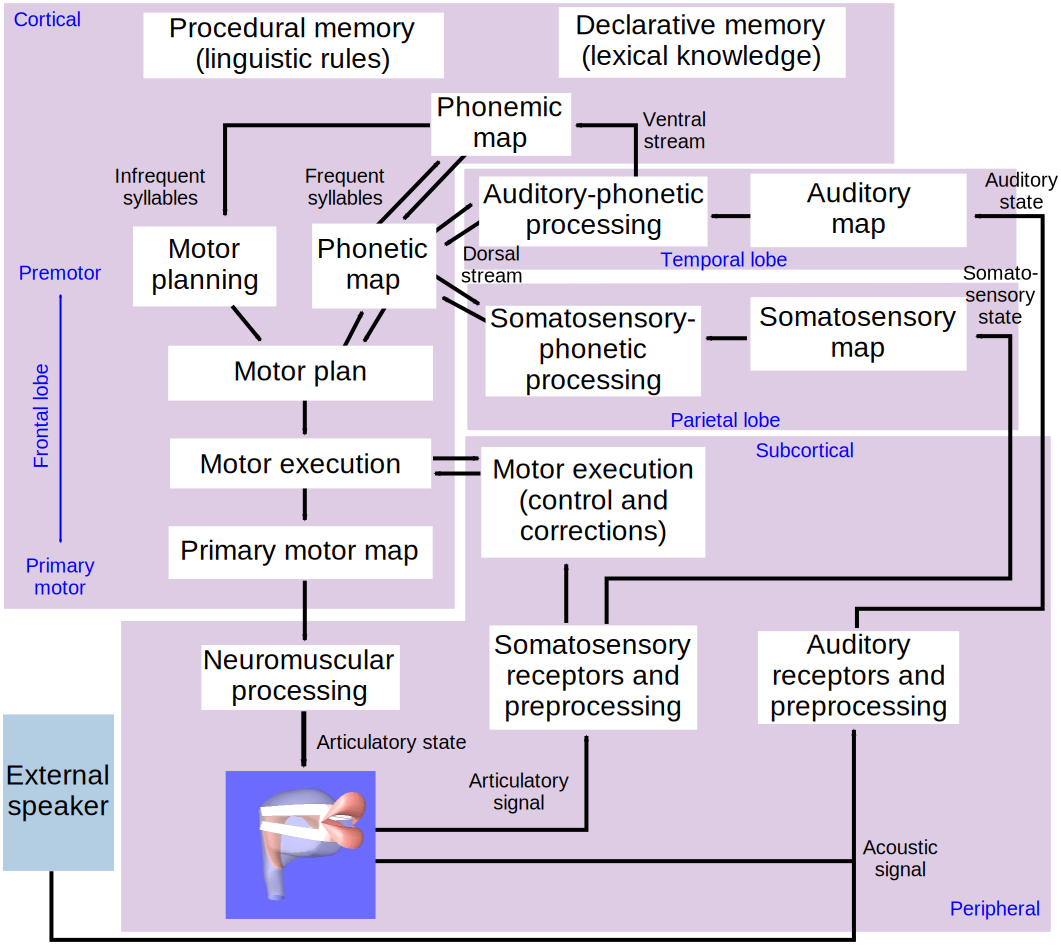
\includegraphics[width=0.8\linewidth]{kroger}
  \end{center}
  \caption{\citeauthor{kroger2009}'s closed loop model
    \citep{kroger2009}.}
  \label{fig:kroger}
\end{figure}

\citeauthor{kroger2009}'s model
is hierarchical; high-dimensional information
reduced to a lower-dimensional representation
using maps.
Similar hierarchies have been explored
in other projects by members of the
Computational Neuroscience Research Group
(e.g., \citealp{eliasmith2012,dewolf2011}).

Other closed-loop models
have been proposed
that use auditory feedback
to learn how to control
an articulatory speech synthesizer.
\citeauthor{warlaumont2012}
developed a spiking neural model
that used a reinforcement-modulated
spike-timing dependent plasticity rule
to reward the firing patterns
responsible for producing
recognizable utterances
in a babbling context
\citep{warlaumont2012,warlaumont2013}.
\citeauthor{howard2011} developed
a model called \textit{Elija}
that goes even further,
starting from babbling
and progressing to learning
the names of objects
(though these objects all had
single syllable names) \citep{howard2011}.
Their focus was on interaction
between a human caregiver
and the model through a microphone.

All three of these closed-loop models
use early childhood acquisition of speech
to test their models,
rather than using feedback
to refine adult speech synthesis.
The only study that I am aware of
that attempts to do closed-loop learning
on a sophisticated articulatory synthesizer
is \citet{prom2013}, which attempted
to minimize the frequency error
between a synthesized and target sound
using a greedy stochastic gradient method.
While they were able to produce
sounds with similar frequency spectrograms
as the target sounds starting from
random initial vocal tract positions
in the Birkholz synthesizer,
the results have not been quantified
and compared to the manual
synthesis techniques.
However, the study does provide
evidence that the Birkholz synthesizer's
control parameters can be learned.

\subsection{Spiking neural networks}
\label{subsec:spiking}

Implementing the previously discussed
biologically inspired techniques in the same way
that biological systems implement
them---i.e., with spiking neurons---may
provide benefits in terms of
computational complexity
(if implemented on massively parallel hardware)
and realism, due to the non-discrete
and noisy nature of biological computation.

Modelling the human auditory system
in spiking neural networks
rarely goes past the periphery,
which has been presented above.
However, studies of
song recognition and production
in songbirds has resulted in
detailed models well grounded in biology,
which may be analogous
to human speech recognition and production.
One key finding in this literature
is that a pathway in the avian brain
that is analogous to
the cortex-basal ganglia-thalamus loop
is active during song learning,
but not production,
just as we might expect
for a general well-trained motor action
in the human brain
(see Figure~\ref{fig:birdsong}).
Spiking neural models have been proposed
in the context of this pathway
that produce sequences of firing patterns,
as observed in the avian brain.

\begin{figure}
  \begin{center}
    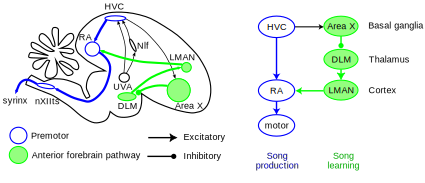
\includegraphics[width=0.85\linewidth]{birdsong}
  \end{center}
  \caption{Neuroanatomy of the avian song learning and production system.
    The \textbf{premotor pathway} is responsible for song production.
    The \textit{HVC} (not an acronym, but sometimes referred to as the
    High Vocal Center) receives input from peripheral auditory nuclei
    and recurrent activity from motor areas;
    it communicates a temporal sequence to the
    \textit{RA} (premotor nucleus) which projects to the
    \textit{nXIIts} (a part of the hypoglossal nerve),
    which controls muscle contractions in the syrinx
    (the syrinx produces sounds and is analogous
    to the human larynx).
    The \textbf{anterior forebrain pathway} is responsible for
    song learning.
    This pathway also begins with the \textit{HVC}.
    The sequence projects to \textit{Area X},
    which is a homologue to the human basal ganglia.
    Similar to human neuroanatomy,
    Area X projects to \textit{DLM}
    (dorsolateral medial thalamus; thalamus homologue),
    which projects to \textit{LMAN}
    (lateral magnocellular nucleus of anterior neostriatum;
    cortex homologue).
    The LMAN links the learning and production systems
    through projections to the RA.
    Adapted from \citet{fiete2008}.}
  \label{fig:birdsong}
\end{figure}

These firing sequences become
a learned \textit{template} of the song.
The bird then attempts to mimic the song
by producing songs until it matches
the template song;
this process occurs without
external feedback,
suggesting that it is trying
to match the learned template specifically.
Models of this template-matching
typically do some type of neurally
implemented reinforcement learning
(e.g., \citealp{fiete2007}).

Both of these processes---sequence generation
through a cortex-basal ganglia-thalamus loop,
and reinforcement learning in the same context---have
been explored by members of the CNRG,
specifically in this case by
the proposer of this research
\citep{stewart2012}.

While these spiking models
replicate avian experimental results well,
we are aware of only one study that
has extrapolated these models
to the domain of human speech:
\citet{yildiz2013} used a birdsong
circuit to do speech recognition
with an error rate comparable
to the HMM-based methods described previously.
However, the vocabulary of words was very small
(10 words, uttered by several different speakers),
and the model used a neuron model
that produced firing rates rather than spike times.

\subsubsection{Neural Engineering Framework}
\label{subsec:nef}

The Neural Engineering Framework (NEF; \citealp{eliasmith2003})
provides a set of tools to integrate
the previously described
spiking neural models,
statistical models,
and control theory models.
The NEF defines three principles
through which to represent
information in spiking neural networks,
transform that information through the connections
between populations of spiking neurons,
and implement dynamics through
recurrent connectivity.

Implementing these models
in the NEF ensures that all
of the models can be integrated together
and allows for more flexibility
than traditional spiking neural networks,
as the principles do not depend
on a particular neuron model.
Firing rate approximations
and direct differential equation integration
can be used to validate models
before running a computationally intensive
spiking neuron simulation.

An important benefit to using the NEF
is that known transformations
(e.g., routing information from one area
to another, or inverse Fourier transforms)
can be optimized offline,
while unknown transformations
(e.g., the mapping from a waveform
to a phoneme)
can be learned online.
An important downside to using the NEF
is additional complexity
in constructing models,
and additional computational complexity
in simulating models.

\subsubsection{Learning}
\label{subsec:learning}

As mentioned above, known transformations
are implemented in the NEF by solving
an optimization problem
that results in a set of connection weights
between two neural populations
that implements the desired transformation.
Unknown transformations are learned
online with a learning rule
that minimizes an arbitrary error signal
\citep{macneil2011}.

The learning rule is
\begin{equation}
  \Delta \omega_{ij} \propto \alpha_j \mathbf{e}_j \cdot \mathbf{E} a_i,
\end{equation}
where $\Delta \omega_{ij}$ is the change in
the connection weight between
a presynaptic neuron indexed with $i$
and a postsynaptic neuron index with $j$,
$\mathbf{e}_j$ describes the type of signals
neuron $j$ is sensitive to,
$\alpha_j$ describes how sensitive
it is to that signal,
$\mathbf{E}$ is the error signal being minimized,
and $a_i$ is the activity of neuron $i$.
This learning rule can be thought of
as a type of gradient descent learning
similar to back-propagation,
except that rather than using
derivatives to determine which
neurons are responsible for the overall error,
this rule uses the similarity (i.e., dot product)
between the overall error, $\mathbf{E}$,
and the part of the vector space
that the neuron is sensitive to, $\mathbf{e}_j$.

Previously, I have combined that rule
with an unsupervised learning rule
and showed that the error minimization
can be done more effectively with
the unsupervised component
\citep{bekolay2013}.
Other members of the CNRG,
have recently experimented
with other unsupervised rules
and implemented them
in a more scalable and efficient manner
(E. Crawford, personal communication).

\section{Proposal}
\label{sec:proposal}

The reviewed background
provides an optimistic long-term
goal for a biologically plausible
model of the speech system,
from the activity of sensory
hair cells in the ear
to the activation of
the muscles in the vocal tract.
Such a system would involve
a recognition hierarchy,
taking in high-dimensional auditory features
and mapping them to lower-dimensional
features like word sequences
and prosodic characteristics,
and a synthesis hierarchy,
mapping from the lower-dimensional
linguistic and prosodic features
to continuous control signals
manipulating high-dimensional parameters
of a simulated vocal tract.

\begin{figure}
  \begin{center}
    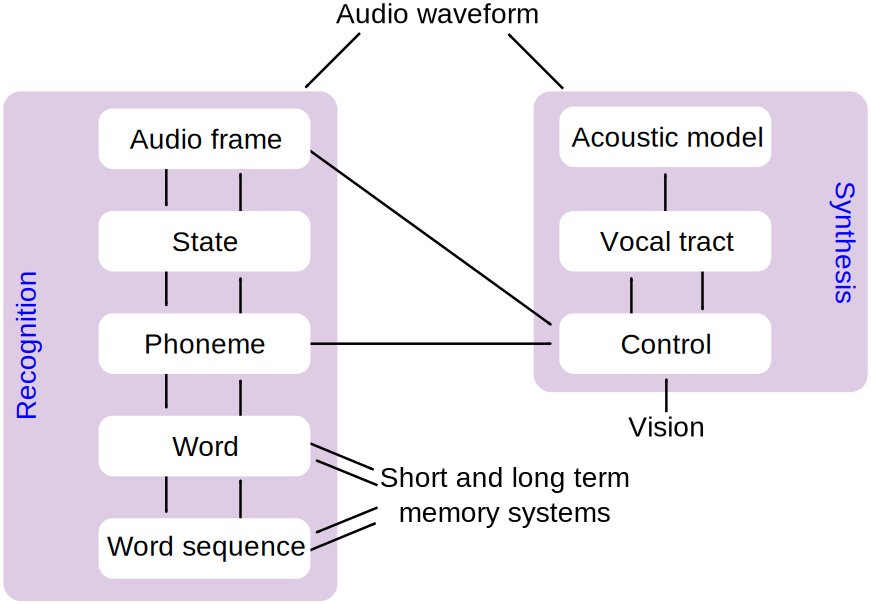
\includegraphics[width=0.7\linewidth]{longterm}
  \end{center}
  \caption{Long-term goal of this line of research: a system consisting
    of interacting recognition and synthesis systems,
    allowing for human-like interaction with an artificial system.}
  \label{fig:longterm}
\end{figure}

Having both of these hierarchies
in a single unified system
allows for many feedback connections,
both within each hierarchy
and between them.
For example, within the recognition hierarchy,
word sequences could be fed back through
the hierarchy to generate
the phoneme sequence corresponding
to that word sequence,
which may be a better representation
to send to the control system.
Word sequences can
be stored in short term memory
while being uttered.
While the phoneme may be
generating the control signal,
the audio frame that results from
the voiced utterance can be compared
to the desired utterance
to improve control.

This type of large-scale unified system
is a good long-term goal,
but is not a reasonable
goal in the span of a PhD.
My PhD project is a subset
of that long-term goal.
It requires the interaction of both hierarchies,
and it can serve as a starting point
for future work towards a large-scale
unified model of human speech.

\subsection{Recognizing and articulating a small vocabulary}
\label{subsec:proposal}

The goal of my PhD project is to
use a speech recognition system
to recognize a small vocabulary of words
(for example, the ten digits)
and use the recognized and remembered
speech samples to train
an articulatory synthesizer
to voice the same small vocabulary.
The main challenges in this project
are determining how to connect
existing systems together
and choosing representations that
can be communicated between systems.
The primary contribution of this project
is a method to train an
articulatory synthesizer
to voice a small vocabulary
without requiring a large corpus
of experimental data
in order to determine appropriate control signals.

\begin{figure}
  \begin{center}
    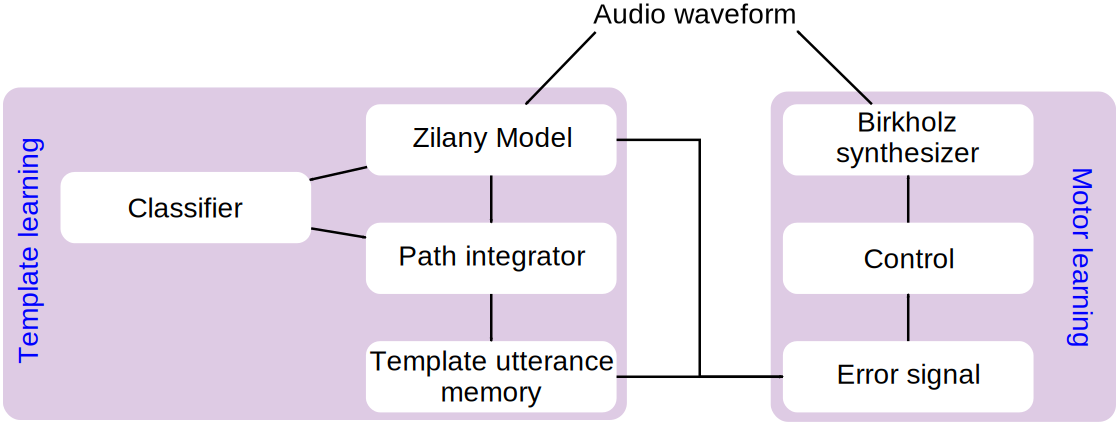
\includegraphics[width=0.7\linewidth]{shortterm}
  \end{center}
  \caption{Short-term goal of this line of research:
    a system consisting of interacting
    recognition and synthesis systems
    that recognizes a small vocabulary of words,
    remembers them, and trains itself to voice
    that same vocabulary with no prior knowledge.}
  \label{fig:shortterm}
\end{figure}

Figure~\ref{fig:shortterm} proposes a system that
achieves the goal of recognizing
and articulating a small vocabulary.
This implementation is inspired by
how songbirds learn to voice
learned songs
(as summarized in Section~\ref{subsec:spiking}).
In the first stage, the words from
the vocabulary are fed to the
recognition hierarchy.
The job of the recognition hierarchy
is to classify the incoming
audio waveforms into the word
being voiced,
and to build up a representation
of what those words sounds like;
we will refer to this as
\textit{template learning},
borrowing the terminology
from the birdsong literature.
In the second stage, the templates
are used to train the
synthesis hierarchy.
The job of the synthesis hierarchy
is to voice the learned template words
as accurately as possible.
This will be done by replaying
the learned templates and
exploring the control parameter space
to determine control signals
that will match the learned templates;
we will refer to this as
\textit{motor learning}.

\subsubsection{Template learning}
\label{subsec:template-learning}

We propose a template learning system
with three key components.
The first component is the Zilany
auditory periphery model,
which we will use as a frontend
to extract auditory features
from the input waveform.
The Zilany model is described in more detail
in section~\ref{subsec:zilany}.
While it has not yet been shown
that the Zilany model produces features
that make recognition
easier or more efficient,
we believe that using a model
that produces spikes
(which can be converted into
instantaneous rates if desired)
leaves open more possibilities
for future model extensions.
The second component of the model
is a classification system
that categorizes auditory features into words,
and the third component
is a path integration system
to remember and replay the
remembered auditory features
for each word in the vocabulary.

The classification system will be based
on my previous work.
In \citet{bekolay2013}, we used visual features
of digits to classify them
using a biologically plausible learning rule
operating in a spiking neural network
created using the principles of the NEF.
In this work, we will use auditory features,
which (unlike the visual features used previously)
change over time.
While we believe that temporal information
will improve the accuracy of classification,
incorporating temporal information
into the existing system will be a challenge.

The path integration model will be based
on an existing line of models
developed by \citet{conklin2005}
and an ongoing extension
by Trujillo (unpublished).
In these path integration models,
a population of neurons tracks
the spatial location of the subject
over time.
In this work, we will track
auditory features over time
instead of spatial location.
The \citeauthor{conklin2005}
model scales up naturally
to arbitrary dimensionality,
so the model should not need
significant modifications.

With these three systems,
we propose a
two stage template learning system.
In the first stage,
we train the classification system
to recognize spoken digits
given the auditory features
produced by the Zilany model.
Once digits can be accurately classified,
we move to the second stage
in which we build up a path through
auditory feature space for each digit.
Upon hearing a new utterance,
the classification system
would determine the digit being uttered;
the path integration system
will then replay the auditory features
of that digit utterance
and incorporate it into
a ``template'' digit utterance,
which would be similar to the
average of all utterances
the system has heard
of that particular digit.

An important possible extension to
this template learning system
(which is not part of the proposed work)
is to make each learning stage hierarchical.
The proposed system is likely
to work well for a small vocabulary,
but it is unlikely to scale up to
a human-scale vocabulary.
Instead, it is likely that
early learning will occur this way
(by mapping from auditory features to words),
but later on we develop a hierarchical mapping
from auditory features to phonemes,
which in turn maps to parts of words or words.
This would allow for fast learning
of new words by integrating
a path through phoneme space
instead of auditory feature space.

\subsubsection{Motor learning}
\label{subsec:motor-learning}

The goal of the motor learning system
is to control the Birkholz articulatory synthesizer
such that it can match
the template digit utterances learned
by the template learning system.
Unlike other control models, however,
this system will start with
no prior knowledge
of the ``correct'' articulator positions
(through MRI data, for example),
and will instead learn
to produce the target sounds
through auditory feedback.

The motor learning system will
attempt to match the learned template
through repeated trials.
On each trail,
a control signal is generated,
which controls the Birkholz
articulatory synthesizer.
The audio waveform produced
by the synthesizer is fed
to the Zilany auditory model,
and the auditory features
of the synthesized sound
are compared to the template sound
to produce an error signal.
The motor system attempts
to minimize this error signal
on each subsequent trial.
Using methods from
reinforcement learning,
we will explore the control parameter space
and find a suitable trajectory
through that space
such that the error is minimized,
which occurs when the synthesizer
utters something that closely matches
the remembered template utterance.
Much like the path integration system
is remembering a trajectory through
auditory feature space,
rather than physical space,
this reinforcement learning system
is learning a trajectory through
articulatory parameter space,
rather than physical space.

Reinforcement learning in the high-dimensional
articulatory parameter space
is unlikely to be tractable.
I will explore several ways to speed up
the learning process.
The first speedup is to prematurely end trials
if a certain amount of error has accumulated.
A significant amount of learning time will
be devoted to producing the first correct phoneme,
and so it is more efficient to continually
attempt to voice that phoneme
than it is to continually attempt to voice
all of the phonemes.
Additionally, if that phoneme is not voiced properly,
any sounds produced from that point on
may not be voiced in the correct context;
for example, the vocal tract is in a certain
configuration before voicing the \textit{n}
in o\textit{n}e than before
voicing the \textit{n} in a\textit{n}.
Learning to voice a certain phoneme incorrectly
may need to be unlearned.
The second speedup is to constrain the learning
by fixing visible articulators to be
the correct values during articulation.
Some articulators like lip and jaw positions
can be determined visually,
and it is plausible that when attempting
to match remembered templates,
those articular positions are also
remembered and replayed.
The third speedup is to
do pretraining to determine
how changing each control parameter
affects the resulting audio waveform.
This can be done independent
of the desired target signal;
the goal would be to determine
the effect of moving a single articulator
on the audio waveform being generated.

As with the template learning system,
and important extension of this work
would be to learn to voice
the utterances in a hierarchical manner.
Rather than learning
to utter each template digit,
a hierarchical system would instead
learn how to utter each phoneme,
and plan trajectories through phoneme space.
However, for the small vocabulary proposed,
we predict that this is not necessary.

\section{Conclusion} \label{sec:conclusion}

In this proposal,
we have provided an optimistic long-term goal
for a human speech system,
which uses two interacting hierarchies
to recognize and synthesize speech.
We have proposed to create a smaller system
that makes use of a minimal skeleton
of the full human speech system
in order to recognize and synthesize
a ten word vocabulary.

\subsection{Challenges} \label{subsec:challenges}

The primary challenge in the proposed system
is to connect all of the
systems combined in this work.
As seen in Figure~\ref{fig:shortterm},
seven systems must communicate together
through some protocol.
To ease communication,
all of these systems will be implemented
through a dynamical systems description
that can be implemented
in a spiking neural network.
While five of the seven systems
(all but the Zilany model
and Birholz synthesizer)
have been expressed in this way
in the past,
communicating with the remaining two systems
may present challenges depending on
implementation details.

Within these systems,
necessary modifications provide
additional challenges.
In the classification system,
temporal information
must be incorporated in
a system that has been used
to classify static vectors.
Temporal classification
of audio signals
has been done previously using
recurrent neural networks
\citep{graves2006};
these methods will be
incorporated into the existing
classification system.

Some of the proposed systems
can be trained in different ways
that will impact their efficiency and effectiveness.
In the classification system,
the easiest training method
is to give the classifier
the correct label during the training phase.
However, the biological plausibility
of such a training scheme is questionable.
One alternative would be to
use approximate labels;
i.e., instead of just using a label,
have that label be bound together
with some random information.
Another alternative would be
to do completely unsupervised learning,
and hope that the words in the vocabulary
are far enough in auditory feature space
to be modeled with some kind of
unsupervised learning.
In the motor learning system,
we have proposed to learn to voice
the first phoneme and then each
subsequent phoneme serially.
However, it may be the case that
learning different subsets
of the auditory sequence
will be beneficial.
Additionally, it may be the case
that it is not possible
to learn a good trajectory
through control parameter space
with no prior knowledge.
In that case, we can bootstrap the system
with existing control methods.

\subsection{Contributions}
\label{subsec:contributions}

Speech recognition and synthesis
are problems that have been worked
on for half a century in both academia and industry;
achieving lower error rates
than state of the art recognition systems
and producing speech that sounds as natural
as systems that use a huge corpus
of recorded speech are
difficult goals to achieve.
The primary contribution of the proposed work
is not to improve on the state of the art,
but to integrate multiple systems together
such that, in the future,
state of the art systems
can be combined together
to improve one another.
Part of achieving this goal will involve
integrating many systems together,
most using the NEF to represent
and transform information.
By doing this, we also wish to show
that implemented biologically inspired methods
in a neural architecture
can provide quantifiable benefits
in terms of parallelizing expensive computations
and reducing the number of data conversions
that have to occur.

While making the best recognizer or synthesizer
is not our explicit goal,
this work will still make contributions
to speech recognition and synthesis individually.
On the recognition side,
we will be the first to use
the Zilany model as a frontend
to a speech recognition system.
While all frontends attempt to
replicate the function of the human ear,
the Zilany model replicates it
to the point that it is used
in cochlear implants.
It may be an ideal frontend
to a speech recognition hierarchy.
On the synthesis side,
articulatory synthesizers
have a long history,
yet still cannot be optimally controlled.
Providing a method for
optimal or near optimal control
of arbitrary articulatory synthesizers
will enable apples-to-apples comparisons.
At the moment, articulatory synthesizers
are difficult to compare to one another
because they depend partly
on how well they are being controlled.
However, with a good control method,
synthesizers can be evaluated
for the quantitative error between
a target utterance
and the synthesized version
in the ideal case of optimal control.

\bibliographystyle{abbrvnat}
\bibliography{proposal}

\end{document}
